% !TeX root = ../thuthesis-example.tex

% Your chapter title here
% Please make sure that the title is in CAPITALS
% All section and subsection headings, use capital letters where required
\chapter{INTRODUCTION}

\section{Problem definition}

Internet of Things (IoT) is expected to connect hundreds of billions of devices in less than a decade\cite{simiscuka_synchronisation_2018}, with tens of billions of connected IoT devices already exist in the world, and this number is anticipated to keep increasing as the Internet connectivity has become a standard feature for a great number of electronic devices\cite{hu_virtual_2021}. Many companies, such as Huawei, Baidu, Alibaba, Tencent, Google, Intel, and so on, already provide their solutions for operating with data coming from IoT devices. Although most of the solutions by companies are restricted to be used only with the limited types or models of IoT devices, nonetheless, they may come to the standardization of IoT devices in the next few years. Even nowadays, most of the consumer IoT devices can be controlled by popular smart assistants, such as Apple Siri, Amazon Alexa, Tencent Xiaowei, and others, or by SDKs, such as Apple HomeKit, which makes it possible to control the devices using our phones, computers or Smart Speakers.

On the other hand, controlling the IoT devices through proprietary buttons, screens, sliders located on ones, by smartphones or by smart speakers does not still provide the best user experience. The interaction techniques are very limited: even though the processing power per energy consumption has increased dramatically, and it is possible to have the processing power of high-performance PC of the 1990s in tiny devices, such as smartwatches, there is no freedom of movement and data sharing. Even though 5G networks partly solve the issue, for example by making it possible to create Internet of Vehicle (IoV), the transmission bandwidth is still limited, causing serious safety consequences\cite{hu_virtual_2021}. For example, when computations for interaction techniques, such as hand gesture recognition can not be performed on the IoT device due to its limited computing power, the sensing data can be transferred to the server, analyzed, and only after sent back to the sensing device to provide output for the user.

The sixth generation (6G) mobile network is expected to cast high-speed and high-efficiency transmission standards to adapt to the further development of new applications \cite{liao_information-centric_2021} \cite{huang_survey_2019}. It is expected for 6G network to be an evolution of 5G network, and, therefore, provide faster data sharing between the devices, which will help to overcome the issues stated in the previous paragraph. As soon as it becomes possible, the companies, which adapt their solutions for the new standards faster, will be more successful in the IoT market. This leads to the assumption that the speed of the development in this case is one of the most important factors.

Currently, the common way of integrating IoT devices in the development stage inside the existing environment is to either use their virtual (or digital) twins or by using their prototypes. In the first case, interaction with such devices is performed through a 2D interface, with a very rough simulation of the user behavior, which leads to further underestimations. In the second case, creating a prototype requires waiting for the modeling of the IoT device, sending the schemes to the manufacturers, and then waiting for the prototype to be delivered. In both cases, the disadvantages lead to the possibility of losing the market, either because of lack of usability or because of being too late to enter the market, already taken by the competitors. Companies and researchers need a devoid of these disadvantages instrument, to integrate prototypes of devices inside the existing real-world IoT environment.

In this study, one of this problem solutions is proposed: a platform for developing new IoT devices. In the next section it is described how using another perspective technology can help to create the platform defined above.

\section{Research idea and tasks}

The problem of defining an instrument for having research on the new types of IoT devices and integrating such devices inside the existing real-world environments, which was introduced in the previous section, requires a solution, which can provide, at first, integration of real-world devices, and, at second, interaction with virtual devices.

Similar to IoT, Virtual reality (VR), together with AR, is considered as one of the most important high-throughput application-level requirements of 6G. . Biggest companies, such as Facebook, invest billions in research for AR and VR, with almost a fifth of the company employees working on research in this field (link: https://www.theverge.com/2021/3/12/22326875/facebook-reality-labs-ar-vr-headcount-report TODO: put in the references). Research papers on applying Virtual reality into almost every field can be found, such as games, education, healthcare or industry.

Companies selling Virtual Reality Headsets provide powerful APIs for integration of their devices inside different 3D engines, \footnote{The Virtual reality  market and 3D engine to be used in the research are further discussed in the next chapter.} which can be used for creating an interaction platform with the virtual IoT devices.

The research idea is to integrate Virtual reality headset into IoT environment. In the 6G era, it will be possible to send large amount of data with much smaller latency and much higher speed compared to the speed of 5G networks. For local scenarios, Wi-Fi 6 (802.11ax standard) already provides acceptable results for streaming high- quality video from VR headset to the server.

Nevertheless, only using Virtual reality headsets does not solve the issue defined in the previous section. The research task is to define a layer between real-world IoT environment and user as a researcher to construct new IoT devices. 

\begin{figure}
  \centering
  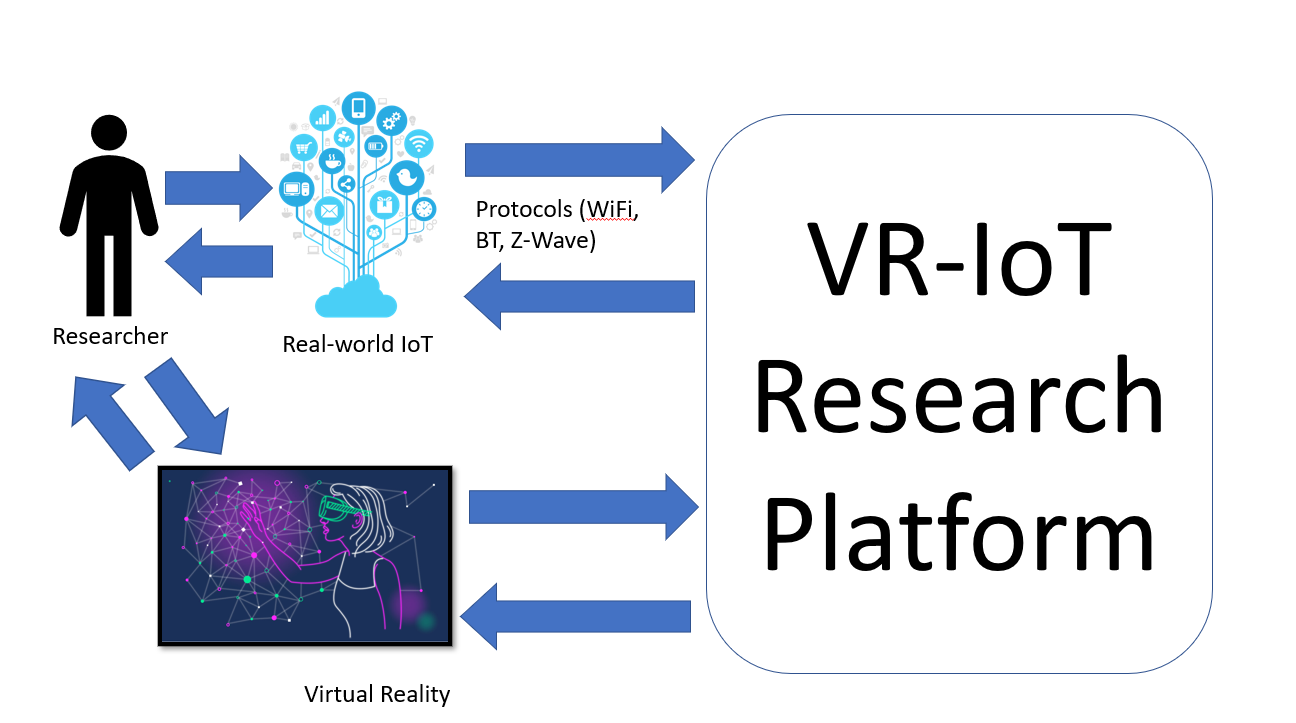
\includegraphics[width=0.9\linewidth]{figures/VR-IoTResearchPlatformLayer.png}
  \caption{VR-IoT Research Platform layer}
  \label{fig:VR-IoTResearchPlatformLayer-figure}
\end{figure}

Since the task is to define the platform, the implementation of the platform can be performed in the future. Nonetheless, as described in the chapter 3, the prototype has been created, with an evaluation in chapter 4, which led to important assumptions on how the platform should be designed in terms of architecture and API for connecting to the real-world IoT devices and Virtual Reality.

Summarizing the problem definition and research task stated previously:

\begin{itemize}
    \item Problem definition: There is no instrument for fast creating, testing and integrating new IoT devices inside an existing real-world environment,
    \item Research task: Define a layer between real-world IoT devices and Virtual Reality. Create a prototype, evaluate the performance and usability and summarize the outputs to explain why the selected architecture can be used as the basis for the future product. (TODO: maybe change the description of the research task)
\end{itemize}